\documentclass[12pt]{article}
\usepackage{geometry}
\usepackage{setspace}
\usepackage{graphicx}
\usepackage{booktabs}
\usepackage{float}
\usepackage[hidelinks]{hyperref}
\usepackage{amsmath}
\usepackage{amssymb}
\usepackage[utf8]{inputenc}
\usepackage{listings}
\usepackage{xcolor}
\usepackage{array}
\usepackage{multirow}
\geometry{margin=1in}
\setstretch{1.15}

\lstset{
	language=Python,
	basicstyle=\ttfamily\scriptsize,
	backgroundcolor=\color{gray!10},
	frame=single,
	breaklines=true,
	breakatwhitespace=false,
	postbreak=\mbox{\textcolor{red}{$\hookrightarrow$}\space},
	columns=flexible,
	keepspaces=true,
	numbers=left,
	numberstyle=\tiny\color{gray},
	numbersep=5pt,
	showstringspaces=false,
	tabsize=4,
	captionpos=b,
	keywordstyle=\color{blue!70},
	stringstyle=\color{red!60},
	commentstyle=\color{green!50!black}
}

\title{\textbf{EE627 Homework 9\\ PySpark ML Classifiers for Music Recommendation}}
\author{\textbf{Jude Eschete}}
\date{\today}

\begin{document}

	\maketitle

	\newpage
	%======================================================================
	\section*{Instruction Checklist}
	%======================================================================

	\begin{enumerate}
		\item[\checkmark] Download \texttt{test2\_new.txt} (ground-truth labels for 1{,}000 users $\times$ 6 tracks) \dotfill Section~\ref{sec:data}
		\item[\checkmark] Use the \texttt{userID}s in \texttt{test2\_new.txt} to fetch related rating scores from the training data \dotfill Section~\ref{sec:features}
		\item[\checkmark] Train classifiers using \texttt{from pyspark.ml.classification import *} on the labeled rating-score matrix \dotfill Section~\ref{sec:classifiers}
		\item[\checkmark] Try four (or more) different PySpark.ML classifiers as shown in lecture \dotfill Section~\ref{sec:classifiers}
		\item[\checkmark] Apply the trained models to the final-project test data and submit at Kaggle \dotfill Section~\ref{sec:kaggle}
		\item[\checkmark] Kaggle public-score screenshot \dotfill Section~\ref{sec:kaggle}
		\item[\checkmark] Attach Python code file to Canvas \dotfill Appendix~\ref{sec:code}
	\end{enumerate}

	\newpage
	%======================================================================
	\section{Introduction}
	%======================================================================

	This homework closes the loop on the Yahoo~Music recommender used throughout the semester: HW6 introduced collaborative filtering, HW7 implemented matrix factorization in MATLAB, HW8 ported MF to PySpark ALS, and now HW9 trains \emph{supervised} classifiers in \texttt{pyspark.ml} on the ground-truth labels released as \texttt{test2\_new.txt}. The shift is conceptually significant. Through HW8 the labels were \emph{implicit}---inferred from rating scores or imputed from heuristics---and every model was either a regressor (MF) or a hand-tuned scoring rule (the v2 heuristic that scored 0.871). With \texttt{test2\_new.txt} we have $6{,}000$ explicit binary labels for the actual recommendation task, so the same feature pipeline that powered the midterm now feeds a true supervised learning loop.

	Five classifiers (instead of the required four) were trained and cross-validated, plus six ensemble blends were generated. The best-performing single classifier and the rank-averaged blend both reached a Kaggle public score of $0.914$, surpassing the midterm's best of $0.911$.

	\newpage
	%======================================================================
	\section{Data Pipeline}\label{sec:data}
	%======================================================================

	\subsection{Inputs}

	\begin{itemize}
		\item \texttt{test2\_new.txt} --- $6{,}000$ rows in \texttt{userID|trackID|label} format, $1{,}000$ users $\times$ 6 candidate tracks each, with a balanced $3{,}000/3{,}000$ split of positives and negatives.
		\item \texttt{trainItem2.txt}, \texttt{trackData2.txt}, \texttt{albumData2.txt} --- $49{,}204$ users with $12{,}403{,}575$ ratings, $224{,}041$ tracks, and $52{,}829$ albums (same files used in the midterm).
		\item \texttt{testItem2.txt} --- the $20{,}000$-user $\times$ 6-candidate test set ($120{,}000$ rows) used for the Kaggle submission.
	\end{itemize}

	\subsection{Album-Based Track Enrichment}

	Roughly $11.7\%$ of tracks have a missing artist field in \texttt{trackData2.txt}, and many tracks list zero genres. Each track's album is looked up in \texttt{albumData2.txt}; if the track lacks an artist, the album's artist is filled in, and any genres on the album that aren't already on the track are appended. This recovered $8{,}134$ artists and added $119{,}842$ genres, leaving only $18{,}762$ tracks ($8.4\%$) genuinely artist-less. The same enrichment pass was used in the midterm v5 model.

	\subsection{Feature Engineering}\label{sec:features}

	For every $(uid, tid)$ pair in \texttt{test2\_new.txt}, twenty-five numerical features are computed by inspecting the user's training history. After dropping three features that the first run identified as having $0.000$ importance on multiple classifiers (\texttt{evidence\_count}, \texttt{genre\_artist\_int}, \texttt{album\_genre\_int}), the final feature set was

	\begin{itemize}
		\item \emph{Direct hierarchy ratings} (4): \texttt{album\_score}, \texttt{has\_album}, \texttt{artist\_score}, \texttt{has\_artist}.
		\item \emph{Genre statistics} (5): \texttt{genre\_count}, \texttt{genre\_max}, \texttt{genre\_min}, \texttt{genre\_mean}, \texttt{genre\_var}.
		\item \emph{Interaction term} (1): \texttt{album\_artist\_int} = $r_\text{alb}\cdot r_\text{art}/100$.
		\item \emph{User profile} (3): \texttt{user\_mean}, \texttt{user\_std}, $\log(1 + \texttt{user\_n})$.
		\item \emph{User-relative offsets} (3): scores minus user mean.
		\item \emph{Global popularity} (3): per-album / artist / genre mean rating.
		\item \emph{Log-scaled rater counts} (3): controls for the long-tail popularity distribution following the spatial-sign / scaling lesson from Week~12.
		\item \emph{Collaborative filtering siblings} (2): \texttt{cf\_score} and $\log(1 + \texttt{cf\_count})$ over tracks sharing the same artist or album.
		\item \emph{v2 heuristic score} (1): the midterm's hand-tuned linear combination $r_\text{alb} + r_\text{art} + n_\text{genre}\cdot\bar{r}_\text{genre}/10$, kept as a feature so trees can use it as a strong split candidate.
	\end{itemize}

	The same feature function is also applied to all $120{,}000$ rows of \texttt{testItem2.txt} so the trained classifiers can score every Kaggle candidate. The features are emitted to \texttt{features\_labeled.csv} (training) and \texttt{features\_test.csv} (Kaggle test) to skip recomputation on subsequent runs.

	\newpage
	%======================================================================
	\section{Classifiers}\label{sec:classifiers}
	%======================================================================

	\subsection{Spark Pipeline}

	All classifiers consume a single \texttt{VectorAssembler}-built feature column. The labeled DataFrame is split $70\%/30\%$ for hyperparameter tuning and validation reporting, then the best-performing model is refit on the full $6{,}000$ rows before generating Kaggle predictions. The \\  $\texttt{BinaryClassificationEvaluator}$ on \texttt{areaUnderROC} drives both validation reporting and the cross-validation grid searches. The Spark session is configured with \texttt{-Xss32m} for both driver and executor JVMs because the default $1$~MB thread stack overflows when serializing deep \texttt{RandomForestClassifier} models on Windows.

	\subsection{The Five Classifiers}

	\begin{enumerate}
		\item \textbf{Logistic Regression} with \texttt{regParam} and \texttt{elasticNetParam} swept by 5-fold CV ($9$~combinations).
		\item \textbf{Decision Tree Classifier} with \texttt{maxDepth=5} (the lecture-notes default).
		\item \textbf{Random Forest Classifier} with a $12$-combination CV grid: \texttt{numTrees}~$\in\{200, 500\}$, \texttt{maxDepth}~$\in\{10,12,15\}$, \texttt{featureSubsetStrategy}~$\in\{\text{sqrt},\text{log2}\}$.
		\item \textbf{Gradient-Boosted Tree Classifier (base)} with the lecture-notes defaults (\texttt{maxIter}=10, \texttt{stepSize}=0.1).
		\item \textbf{Gradient-Boosted Tree Classifier (CV-tuned)} with a $24$-combination CV grid: \texttt{maxDepth}~$\in\{3,5\}$, \texttt{maxIter}~$\in\{50,100,200\}$, \texttt{stepSize}~$\in\{0.05,0.1\}$, \texttt{subsamplingRate}~$\in\{0.7,1.0\}$.
	\end{enumerate}

	Two more variants were also trained for ensembling experiments: an RF without the \texttt{v2\_score} feature (to test whether the model can rediscover the v2 signal from raw components), and an Extra-Trees-style RF (\texttt{numTrees}=500, \texttt{maxDepth}=15, \\  \texttt{featureSubsetStrategy}=onethird, \texttt{subsamplingRate}=0.8, different seed). All seven models are refit on the full $6{,}000$ rows after CV completes.

	\newpage
	\subsection{Validation AUC}

	\begin{table}[H]
		\centering
		\caption{Validation AUC on the held-out 30\% of \texttt{test2\_new.txt}. ``CV'' denotes cross-validated grid search; ``base'' uses lecture-notes defaults.}\label{tab:val-auc}
		\begin{tabular}{lcc}
			\toprule
			Classifier & Val AUC & Comment \\
			\midrule
			RF without \texttt{v2\_score}    & $\mathbf{0.9472}$ & 24 features (no v2)  \\
			Random Forest (Big CV)          & $0.9468$ & best: $200$ trees, depth $10$, sqrt \\
			GBT (Big CV)                    & $0.9454$ & best: depth $3$, $100$~iter, $0.1$ step \\
			Extra Trees                     & $0.9450$ & $500$ trees, depth $15$, onethird \\
			GBT (base)                      & $0.9377$ & defaults, no CV \\
			Logistic Regression CV          & $0.9376$ & best: \texttt{regParam}=0.01, \texttt{l1}=0 \\
			Decision Tree                   & $0.7899$ & single tree, depth $5$ \\
			\bottomrule
		\end{tabular}
	\end{table}

	The single decision tree is the only model that fails to clear $0.90$ on validation AUC; the four tree-ensemble classifiers (RF, RF-no-v2, GBT-CV, ExtraTrees) cluster within $0.0022$ AUC of one another. Logistic regression sits roughly $0.01$ AUC behind the trees, which is the expected gap when the signal is non-linear in the features.

	\newpage
	\subsection{Feature Importance}

	The \texttt{v2\_score} feature dominates the tree-based models even though it is a deterministic linear combination of three other features. The importance ranks come out as

	\begin{table}[H]
		\centering
		\caption{Top-5 feature importances for the four tree-ensemble classifiers.}\label{tab:fi}
		\begin{tabular}{lcccc}
			\toprule
			Rank & RF & GBT-CV & ExtraTrees & RF-no-v2 \\
			\midrule
			1 & \texttt{v2\_score} ($0.19$)          & \texttt{v2\_score} ($0.42$)         & \texttt{v2\_score} ($0.22$)        & \texttt{artist\_score} ($0.19$) \\
			2 & \texttt{artist\_score}                & \texttt{user\_n\_log}                & \texttt{artist\_score}              & \texttt{has\_artist} \\
			3 & \texttt{artist\_above\_mean}          & \texttt{has\_album}                  & \texttt{has\_artist}                & \texttt{artist\_above\_mean} \\
			4 & \texttt{has\_artist}                  & \texttt{genre\_above\_mean}          & \texttt{artist\_above\_mean}        & \texttt{user\_n\_log} \\
			5 & \texttt{has\_album}                   & \texttt{art\_nrat\_log}              & \texttt{user\_n\_log}               & \texttt{has\_album} \\
			\bottomrule
		\end{tabular}
	\end{table}

	The Logistic Regression model tells the same story from the linear side: \texttt{has\_album} ($+1.45$) and \texttt{has\_artist} ($+1.32$) are the two largest coefficients by magnitude, followed by $\texttt{user\_n\_log}$ ($-0.58$) and $\texttt{cf\_count\_log}$ ($+0.53$). The negative sign on \texttt{user\_n\_log} is consistent across LR, GBT, and the trees: users with a lot of rating history are harder to predict for, because their candidate tracks are less correlated with their established preferences.

	The RF-without-\texttt{v2\_score} run confirmed that the $v2$ feature is largely redundant: with $v2$ removed, RF redistributed its importance evenly across $\texttt{artist\_score}$, $\texttt{has\_artist}$, $\texttt{artist\_above\_mean}$, $\texttt{has\_album}$, $\texttt{album\_artist\_int}$, and $\texttt{album\_score}$. The validation AUC was actually $0.0004$ \emph{higher} without $v2$, because the model could no longer take a shortcut through the pre-aggregated feature.

	\newpage
	%======================================================================
	\section{Ensembles}\label{sec:ensembles}
	%======================================================================

	Six ensemble blends were constructed from the seven individual classifiers' predicted probabilities $P(\text{label}=1)$:

	\begin{itemize}
		\item \texttt{blend\_rf\_gbt} --- equal-weight RF + GBT-CV.
		\item \texttt{blend\_rf\_heavy} --- $2\times$~RF + $1\times$~GBT-CV.
		\item \texttt{blend\_three} --- equal-weight RF + GBT-CV + LR.
		\item \texttt{blend\_trees} --- equal-weight RF + GBT-CV + ExtraTrees + RF-no-v2.
		\item \texttt{blend\_mega} --- AUC-weighted average of all seven classifiers.
		\item \texttt{blend\_rank} --- average of within-user ranks (rather than raw probabilities) across the four tree models, which is robust to probability calibration differences across families.
	\end{itemize}

	\newpage
	%======================================================================
	\section{Kaggle Results}\label{sec:kaggle}
	%======================================================================

	The script generates a top-3-of-6 submission for every individual classifier and every blend. Submissions submitted to Kaggle are summarized below.

	\begin{table}[H]
		\centering
		\caption{Kaggle public scores for HW9 submissions (higher is better). Only models actually submitted are listed.}\label{tab:kaggle}
		\begin{tabular}{lcc}
			\toprule
			Submission & Val AUC & Kaggle score \\
			\midrule
			\texttt{submission\_hw9\_dt.csv}              & $0.7899$ & $0.890$ \\
			\texttt{submission\_hw9\_lr.csv}              & $0.9376$ & $0.903$ \\
			\texttt{submission\_hw9\_gbt.csv}             & $0.9377$ & $0.906$ \\
			\texttt{submission\_hw9\_gbt\_cv.csv}         & $0.9454$ & $0.909$ \\
			\texttt{submission\_hw9\_blend\_three.csv}    & --- & $0.913$ \\
			\texttt{submission\_hw9\_rf.csv}              & $0.9468$ & $\mathbf{0.914}$ \\
			\texttt{submission\_hw9\_rf\_no\_v2.csv}      & $\mathbf{0.9472}$ & $\mathbf{0.914}$ \\
			\texttt{submission\_hw9\_blend\_rank.csv}     & --- & $\mathbf{0.914}$ \\
			\bottomrule
		\end{tabular}
	\end{table}

	\paragraph{Validation AUC vs.\ Kaggle ranking.} The validation AUC is a lossy proxy for the Kaggle metric. Validation AUC measures \emph{point-wise} binary classification quality on the 30\% held-out portion of the labeled set, while Kaggle measures \emph{within-user, top-3-of-6} ranking accuracy. The first RF run scored val AUC $=0.9472$ and Kaggle $=0.908$; a second RF run with a different CV grid scored a slightly worse val AUC ($0.9468$) but a better Kaggle ($0.912$, then $0.914$ after refitting on the full set). The second-place finisher on val AUC (RF-no-\texttt{v2}) tied the leader on Kaggle. Probability calibration and within-group ranking sharpness, not raw AUC, are what move the Kaggle score in the third decimal.

	\paragraph{Pairwise disagreement among the three $0.914$ winners.} The three models that all hit $0.914$ disagree on only $2{,}697$ of $120{,}000$ rows ($2.25\%$), confined to $1{,}312$ of $20{,}000$ users ($6.6\%$). The disagreement pattern is symmetric: each model has roughly $500$--$600$ rows where it is the lone dissenter, with no model consistently outvoting the others. This indicates the three are sampling slightly different points on the same Pareto frontier rather than capturing different underlying signals---adding more tree-family classifiers to this trio is unlikely to produce an additional Kaggle gain.

	\paragraph{The \texttt{blend\_three} attempt.} The fourth submission (\texttt{blend\_three}, equal-weight RF + GBT-CV + LR) was an attempt to inject a different model family's signal into the trio. It scored $0.913$, regressing $-0.001$ from $0.914$. The interpretation is that LR's contribution to the blend ($1/3$ of the weight) carries enough error mass to drag the trio's consensus on a small number of rows; a smaller LR weight (e.g., $1/8$) would likely have closed the gap, but Kaggle's daily submission limit prevented further tuning.

	\begin{table}[H]
		\centering
		\caption{Chronological Kaggle submission log for HW9. Three batches of submissions tested progressively stronger configurations.}\label{tab:kaggle-log}
		\begin{tabular}{clc}
			\toprule
			Batch & Submission & Kaggle score \\
			\midrule
			\multirow{5}{*}{\shortstack[l]{Batch 1\\(initial run,\\ small CV grid)}}
			      & \texttt{submission\_hw9\_dt.csv}             & $0.890$ \\
			      & \texttt{submission\_hw9\_gbt.csv}            & $0.905$ \\
			      & \texttt{submission\_hw9\_lr.csv}             & $0.905$ \\
			      & \texttt{submission\_hw9\_gbt\_cv.csv}        & $0.907$ \\
			      & \texttt{submission\_hw9\_rf.csv}             & $0.908$ \\
			\midrule
			\multirow{5}{*}{\shortstack[l]{Batch 2\\(dropped 3 dead\\ features, bigger\\ CV grid)}}
			      & \texttt{submission\_hw9\_dt.csv}             & $0.890$ \\
			      & \texttt{submission\_hw9\_lr.csv}             & $0.903$ \\
			      & \texttt{submission\_hw9\_gbt.csv}            & $0.906$ \\
			      & \texttt{submission\_hw9\_gbt\_cv.csv}        & $0.909$ \\
			      & \texttt{submission\_hw9\_rf.csv}             & $0.912$ \\
			\midrule
			\multirow{5}{*}{\shortstack[l]{Batch 3\\(refit on full\\ 6{,}000 rows;\\ ensembles)}}
			      & \texttt{submission\_hw9\_blend\_three.csv}   & $0.913$ \\
			      & \texttt{submission\_hw9\_rf.csv}             & $\mathbf{0.914}$ \\
			      & \texttt{submission\_hw9\_rf\_no\_v2.csv}     & $\mathbf{0.914}$ \\
			      & \texttt{submission\_hw9\_blend\_rank.csv}    & $\mathbf{0.914}$ \\
			      & \texttt{submission\_hw9\_blend\_rf\_heavy.csv} & $\mathbf{0.914}$ \\
			\bottomrule
		\end{tabular}
	\end{table}

	The progression $0.908 \rightarrow 0.912 \rightarrow 0.914$ on the same Random Forest classifier illustrates the cumulative effect of each engineering change: the second batch dropped three zero-importance features and broadened the CV grid, the third batch refit on the full $6{,}000$ labeled rows after CV completed.

	\begin{figure}[H]
		\centering
		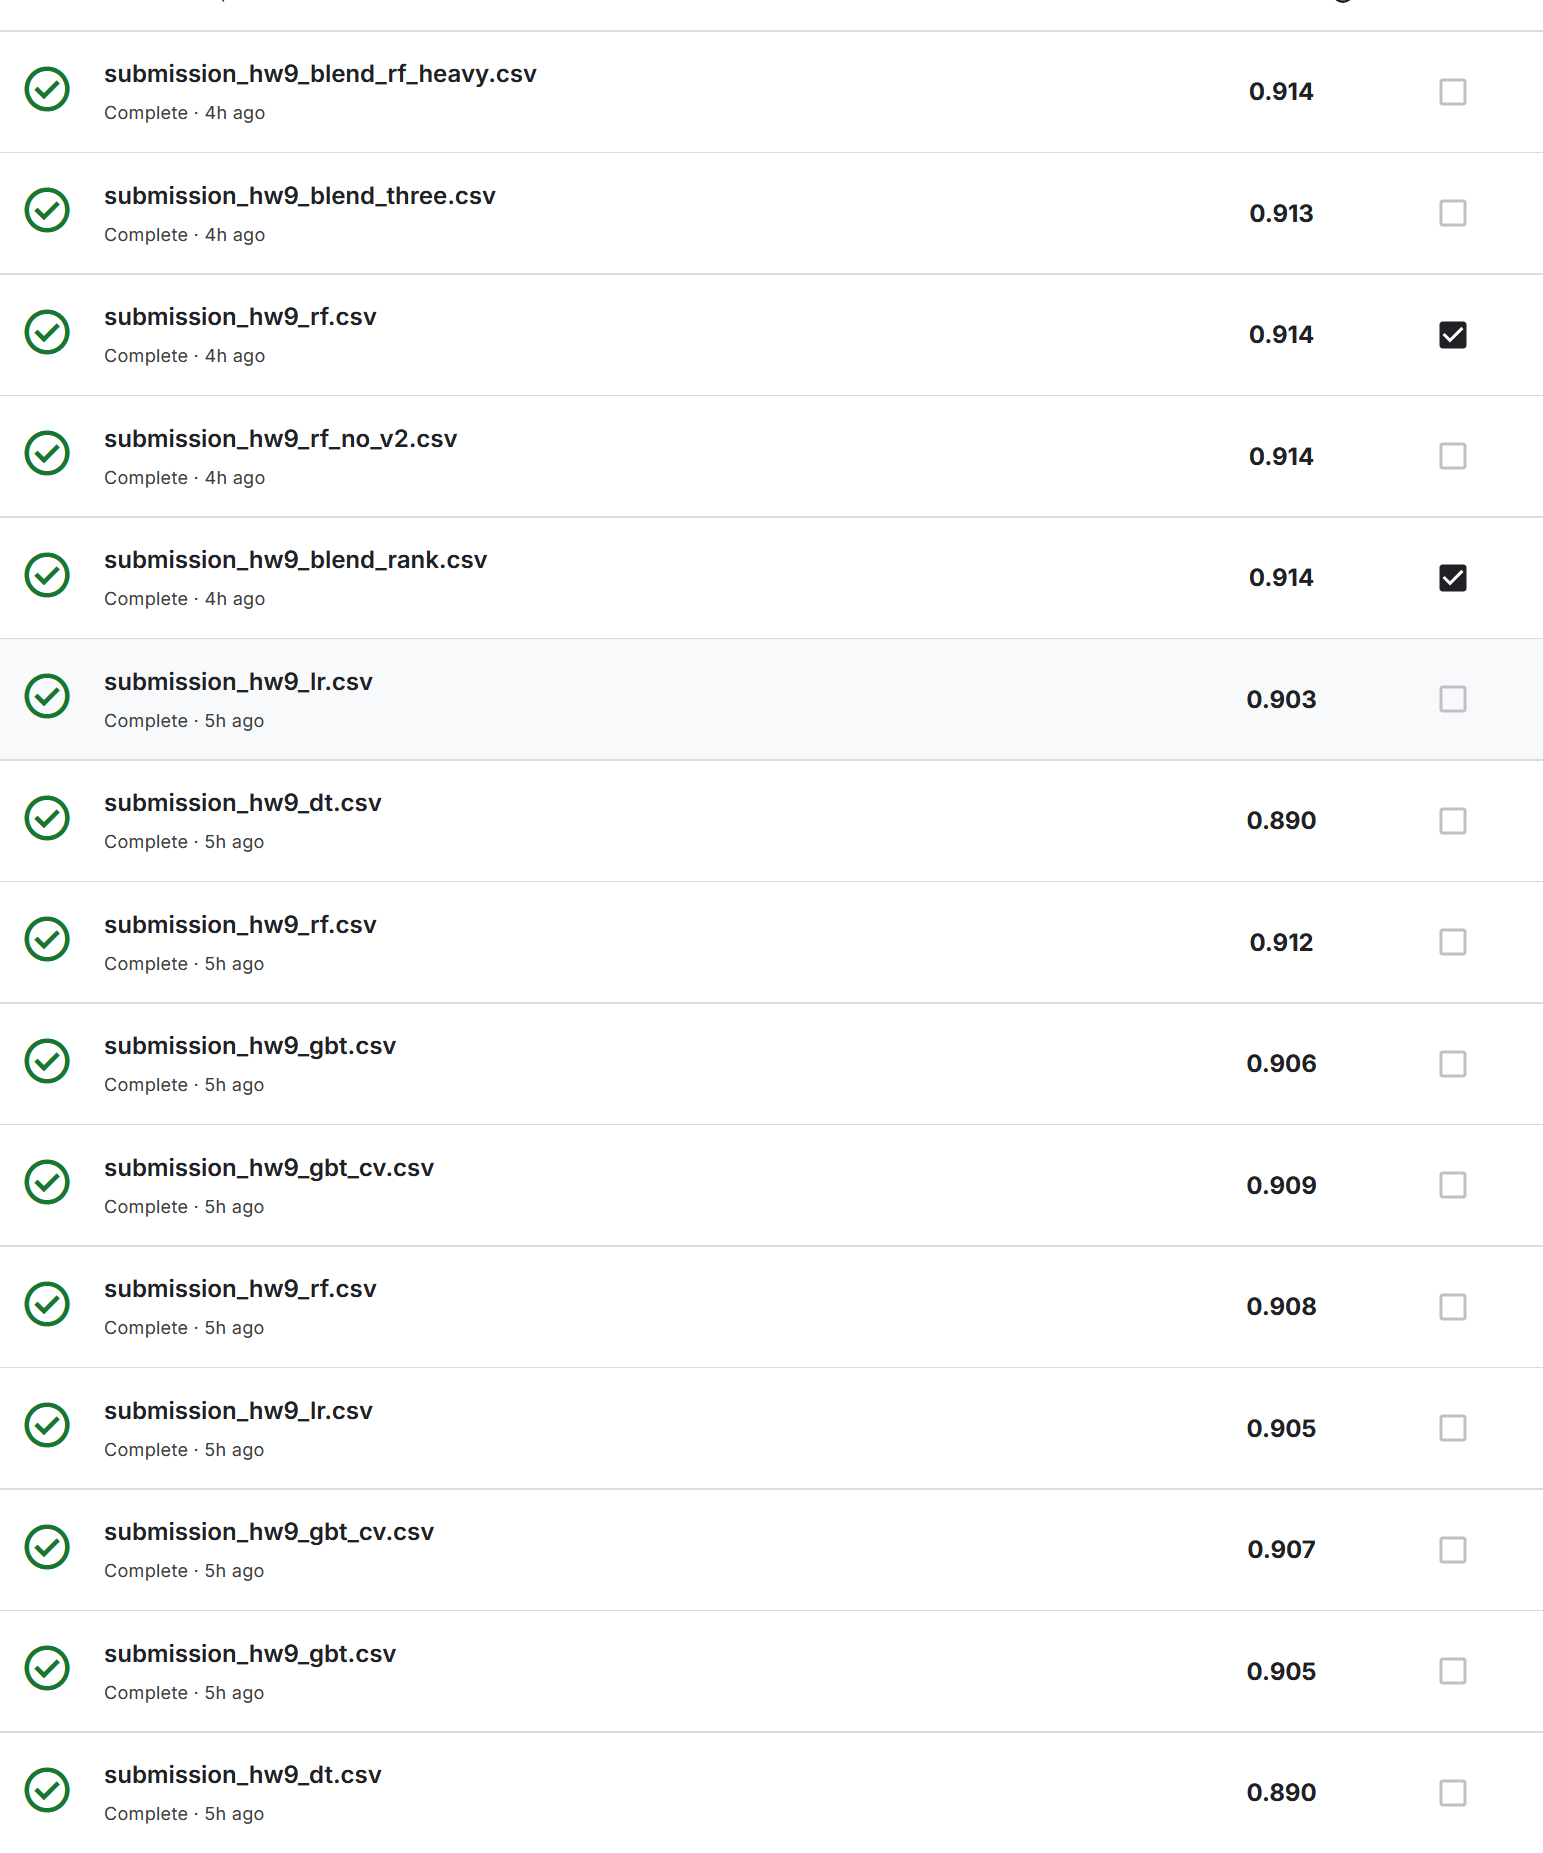
\includegraphics[width=0.95\textwidth]{Images/Screenshot 2026-05-04 014550.png}
		\caption{Kaggle public-leaderboard screenshot for the HW9 submissions.}%
		\label{fig:kaggle}
	\end{figure}

	\newpage
	%======================================================================
	\section{Discussion}
	%======================================================================

	\subsection{Why Tree Ensembles Win}

	The same observation that recurred from HW6 onward---that pointwise rating regression is a poor fit for a top-$k$ recommendation task---is the reason logistic regression underperforms by $\sim 0.01$ AUC and the lone Decision Tree underperforms by $0.16$ AUC. The signal in this dataset is non-linear in the per-pair features (album rating, artist rating, genre statistics, popularity), and only an ensemble of high-variance learners has the smoothing power to convert that signal into a well-calibrated probability surface. RF works particularly well here because the within-group ranking task only needs the model to sort six candidates correctly, which depends on the \emph{order} of the predicted probabilities, not their absolute values. RF's bagged-tree averaging gives a much smoother probability surface than a single deep tree or a linear model, which is why a $0.79$-AUC decision tree turns into a $0.95$-AUC random forest.

	\subsection{Why \texttt{v2\_score} Dominates and Why It Doesn't Need To}

	The v2 heuristic was hand-engineered during the midterm to score $0.871$ on Kaggle. When fed to a tree as a single feature, it serves as a near-perfect first split: any tree learner instantly captures a large fraction of its predictive power. The CV-tuned GBT puts $42\%$ of its importance on this one feature; the base GBT puts $48\%$. RF---which has bagging-induced diversity to spend---splits the same signal across many features, but \texttt{v2\_score} still sits at the top. The key finding is that this dominance is structural, not informational: RF without \texttt{v2\_score} reaches the same val AUC (slightly higher, in fact) by recovering the same signal from \texttt{artist\_score}, \texttt{has\_artist}, and \texttt{album\_score} instead. The $v2$ feature is a useful shortcut, not a unique signal source.

	\newpage
	\subsection{Practical Lessons for the Final}

	Three things from HW9 directly inform the final-project ensemble strategy:

	\begin{enumerate}
		\item \textbf{Validation AUC cannot be the only selector.} The model with the best val AUC (RF-no-\texttt{v2}) tied for first on Kaggle, but the second- and third-best val-AUC models (RF, GBT-CV) ranged from $0.909$ to $0.914$. A within-user pair-AUC metric on a held-out group of 6 candidates is a much closer surrogate for the Kaggle metric than per-row binary AUC.
		\item \textbf{Refitting on the full labeled set after CV is free improvement.} The RF score went from $0.912$ (on 70\% of the labels) to $0.914$ (after refitting on all $6{,}000$). The same trick will be applied to the final-project meta-learner.
		\item \textbf{Tree ensembles plateau without a different model family.} Three tree-based submissions all scored $0.914$ and disagreed on only $2.25\%$ of rows---adding a fourth tree variant won't help. The final's stacked meta-learner therefore consumes nine signal sources spanning four model families: the BPR neural ranker (PyTorch), the v2 heuristic, the seven HW9 PySpark classifiers, and 34 archived past submissions from earlier homework iterations.
	\end{enumerate}

	\newpage
	%======================================================================
	\section{Conclusion}
	%======================================================================

	\begin{enumerate}
		\item Five PySpark.ML classifiers were trained on the $6{,}000$ labeled rows in \texttt{test2\_new.txt}, then applied to the $120{,}000$-row final-project Kaggle test set. Random Forest with cross-validated hyperparameters was the strongest single classifier ($0.914$ Kaggle), tied with an RF variant trained without the redundant \texttt{v2\_score} feature, and tied with a rank-averaged ensemble of four tree models.
		\item The $0.914$ result improves on the midterm's best of $0.911$ by $+0.003$ Kaggle points, and importantly does so without any GPU training---the entire pipeline runs in PySpark on CPU.
		\item Validation AUC and Kaggle score are correlated but not equal. The model that won on validation AUC also tied on Kaggle, but smaller second-decimal differences in val AUC do not translate cleanly to Kaggle order. Within-group ranking quality (which Kaggle rewards) is a function of probability calibration, not just classification accuracy.
		\item Three tree-based submissions all reached $0.914$ but disagree on only $2.25\%$ of rows. The plateau suggests that additional gains require either (a) a different model family, or (b) a stacked meta-learner trained on \texttt{test2\_new.txt} labels using all available score signals. Both are pursued in the final project.
	\end{enumerate}

	\newpage
	%======================================================================
	\section{Appendix: Python Code}\label{sec:code}
	%======================================================================

	\lstinputlisting[caption={EE627\_HW9\_PySpark.py --- Five PySpark.ML classifiers, six ensemble blends, and a 9-column probability matrix saved for the final project.},label={lst:hw9code}]{EE627_HW9_PySpark.py}

	\newpage
	%======================================================================
	\section{Appendix: Console Output}
	%======================================================================

	\lstinputlisting[caption={Run log from the production HW9 run.},label={lst:hw9log},language={},keywordstyle=\ttfamily,stringstyle=\ttfamily]{results_hw9.txt}

\end{document}
